%%%%%%%%%%%%%
% LECTURE 7 %
%%%%%%%%%%%%%
\vspace{1cm}

\noindent\lecture{7}{25/10/2021}
\vspace{0.5cm}
\noindent I prossimi due algoritmi sono tra quelli più conosciuti, in termini di algoritmi quantistici, sia dal punto di vista storico del QC sia dal punto di vista applicativo:
\begin{itemize}
    \item L'algoritmo di ricerca del periodo di una funzione: l'\textbf{algoritmo di Shor};
    \item L'algoritmo di ricerca di particolari elementi in un database: l'\textbf{algoritmo di Grover}.
\end{itemize}
Prima di addentrarci nello studio del più difficile (non vedremo tutto il discorso legato alla teoria dei numeri) dei due, l'algoritmo di Shor, introduciamo il seguente concetto:


\section{Quantum Fourier Transform}
Il cuore dell'algoritmo di Shor è la \textbf{QFT} o \textbf{Quantum Fourier Transform}, che può essere eseguita da un circuito quantistico. La QFT di $n$ qubit è definita come quella trasformazione unitaria $\hat U_{\text{FT}}$ la cui azione su un elemento $\ket{x} \in \mathcal{H}$ è data da:
\begin{equation}\label{QFT}
    \hat U_{\text{FT}}\ket x = \frac{1}{2^{\frac n2}}\sum_{y=0}^{2^n-1}e^{2\pi i\frac{ x \, y }{2^n}}\ket y
\end{equation}
dove con la notazione precedente intendiamo $\ket{x} \equiv \ket{x_{n-1}} \otimes \ket{x_{n-2}} \otimes \ldots \otimes \ket{x_0}$, in cui ciascun qubit $\ket{x_i}$ può essere un elemento della base computazionale, quindi $\ket{0}$ o $\ket{1}$. Notiamo inoltre che il prodotto $x\,  y$ ad esponente è un prodotto  tra interi e non un prodotto bit a bit modulo 2. Lo stato $\ket{x}$ può essere scritto utilizzando anche la codifica digitale degli interi, ossia
\begin{equation*}
    x = 2^{n-1} x_{n-1} + 2^{n-2} x_{n-2} + \ldots + 2^{0} x_0 \, , \; \text{ dove } 0 \leq x \leq 2^n - 1 \, .
\end{equation*}
Notiamo che il fattore davanti alla sommatoria in \eqref{QFT} è un fattore di normalizzazione perché abbiamo diviso per la radice del numero totale degli stati: lo spazio di Hilbert di $\ket{x}$ ha infatti $\dim \mathcal{H} = 2^n$ poiché è frutto del prodotto tensoriale degli $n$ spazi associati ai singoli qubit. Dato che $\hat U_{\text{FT}}$ è un operatore che agisce su $\mathcal{H}$, possiamo applicare la \eqref{QFT} ad una sovrapposizione di stati $\ket x$ con ampiezze complesse $\gamma(x)$:
\begin{equation}
    \label{eq:qtf2}
    \hat U_{\text{FT}} \left( \sum_{x=0}^{2^n-1}\gamma(x)\ket x \right) = \sum_{x,y=0}^{2^n-1} \frac{\gamma(x)}{2^{\frac n2}} e^{2\pi i \frac{x\,y}{2^n}} \ket y = \sum_{y=0}^{2^n-1}\hat \gamma(y)\ket y \, ,
\end{equation}
dove abbiamo ottenuto un'altra sovrapposizione con ampiezze che sono legate a $\gamma(x)$ dalla \textbf{DFT} o \textbf{Discrete Fourier Transform}:
\begin{equation}\label{DFT}
    \hat \gamma(y)=\sum_{x=0}^{2^n-1}\frac{e^{2\pi i \frac{x y}{2^n}}}{2^{\frac n2}}\gamma(x) \, .
\end{equation}
Si noti che la \eqref{QFT} agisce sui coefficienti $\gamma(x)$ come in \eqref{DFT}, ossia tramite una versione discretizzata della trasformata di Fourier standard. In generale la DFT è largamente utilizzata nella teoria dei segnali. 

\noindent Per calcolare ciascun coefficiente $\hat{\gamma}(x)$ in \eqref{DFT} si richiedono $2^n \times 2^n = 2^{2n}$ operazioni (dimensione della matrice), le quali sono un enormità! In CC esiste un celebre algoritmo chiamato \textbf{FFT} o \textbf{Fast Fourier Transform} che migliora il numero precedente fino a $\order{n 2^n}$, ottenendo quindi un modo molto più efficiente per calcolare $\hat{\gamma}(x)$. In realtà esiste un algoritmo quantistico per eseguire la trasformazione unitaria $\hat U_{\text{FT}}$ in un tempo esponenzialmente più veloce, perché cresce solo come $\order{n^2}$. Il problema, come al solito, è che non si può conoscere l'insieme completo dei coefficienti di Fourier, come si fa dopo aver applicato la FFT: il risultato è infatti una sovrapposizione $\sum_y \hat{\gamma} (y) \ket{y}$ sulla quale è necessario effettuare una misurazione che permetterà di ottenere solamente 1 coefficiente. Nonostante quindi l'algoritmo per il calcolo della QFT non migliori l'algoritmo classico della FFT, la \eqref{QFT} si è rivelata molto utile per la risoluzione di problemi del mondo quantistico. Ad esempio, se $\gamma$ è una funzione periodica con un periodo $r$ non maggiore di $2^{\frac n2}$, allora un registro nello stato in \eqref{eq:qtf2} può fornire potenti indizi sul valore preciso del periodo, anche se $r$ può essere lungo centinaia di cifre. Per il momento il nostro scopo è mostrare che è possibile costruire un circuito che calcoli in un numero di step di ordine $\order{n^2}$ la QFT.

\noindent Consideriamo, come al solito, come punto di partenza lo stato $\ket 0^{\otimes n}$. Sappiamo dalla \eqref{n_H_gates} che se applichiamo l'\texttt{H-gate} su tale stato avremo
\begin{equation*}
    H^{\otimes n}\ket{0}^{\otimes n} = \frac{1}{2^{\frac n2}}\sum_{y=0}^{2^n-1} \ket y \, ,
\end{equation*}
ossia una somma su tutti gli stati nella base computazionale. Definiamo ora un operatore $\mathcal{Z}$ che agisce nel modo seguente:
\begin{equation*}
    \mathcal{Z}\ket y = e^{2\pi i \frac{y}{2^n}}\ket y \, ;
\end{equation*}
in questo modo l'operatore $\hat U_{\text{FT}}$ della \eqref{QFT} può essere riscritto come
\begin{equation}\label{QFT_with_Z}
    \hat U_{\text{FT}}\ket x = \mathcal{Z}^xH^{\otimes n}\ket{0}^{\otimes n} = \frac{1}{2^{\frac n2}}\sum_{y=0}^{2^n-1} \mathcal{Z}^x \ket y \, , \; \text{ con } \mathcal{Z} = e^{2\pi i \frac{y}{2^n}} \, ;
\end{equation}
si ricordi sempre che $x$ è un intero. Cerchiamo di capire cosa sia $\mathcal Z$. Consideriamo il caso del qubit singolo ($n=1$):
\begin{equation*}
    \mathcal{Z}\ket y = e^{\pi i y}\ket{y} = 
    \begin{cases}
        \ket{y} \, , &\text{per } y = 0 \\
        -\ket{y} \, , &\text{per } y = 1
    \end{cases}
    \, , \quad \Rightarrow \quad \mathcal{Z} = Z = 
    \begin{pmatrix}
        1 & 0 \\ 0 & -1
    \end{pmatrix} \, .
\end{equation*}
Si noti che un altro modo conveniente di scriverlo è come esponenziale
\begin{equation*}
    Z = e^{i \pi n} \, , \; \text{ dove } n = 
    \begin{pmatrix}
        0 & 0 \\ 0 & 1
    \end{pmatrix} \, .
\end{equation*}
Per passare alla generalizzazione per $n$ qubit ricordiamo che, come lo stato $\ket{x}$ di \eqref{QFT}, possiamo scrivere nella base computazionale che $ \ket y = \ket{y_{n-1}} \otimes \ldots \otimes \ket{y_0}$ e analogamente come intero avremo $y = 2^{n-1} y_{n-1} + \ldots + 2^0 y_0$. Introduciamo $n$ differenti matrici, che chiameremo $n_i$ con $i = 0, \ldots, n-1$, che agiscono sul corrispondente qubit di $\ket{y}$ dando 0 o 1 a seconda del valore del qubit: questo significa scrivere che
\begin{align*}
    \left( 2^{n-1} n_{n-1} + 2^{n-2} n_{n-2} + \ldots + n_0 \right) \ket y &= 2^{n-1} y_{n-1} \ket{y_{n-1}} \otimes \ldots \otimes \ket{y_0} \\
    &\quad + \ket{y_{n-1}} \otimes 2^{n-2} y_{n-2} \ket{y_{n-2}} \otimes \ldots \otimes \ket{y_0} \\
    &\quad + \ldots + \ket{y_{n-1}} \otimes \ldots \otimes y_0 \ket{y_0} \\
    &= (2^{n-1} y_{n-1} + \ldots y_0) \ket{y} = y\ket y \, ,
\end{align*}
quindi si tratta di un particolare modo di calcolare la codifica digitale, ossia l'intero $y$, dello stato $\ket{y}$. Notiamo che la matrice $n_{n-1}$ agisce su $\ket{y_{n-1}}$, $n_{n-2}$ agisce su $\ket{y_{n-2}}$ e così via fino a $n_0$ che agisce su $\ket{y_0}$,   questo perché in generale $n_p \ket{y_p} = y_p \ket{y_p}$. Utilizzando quindi questa notazione possiamo riscrivere l'operatore $\mathcal{Z}$ in questo modo: 
\begin{equation*}
    \mathcal{Z} \ket y = e^{\frac{2 \pi i}{2^n} y} \ket y = e^{\frac{2\pi i}{2^n} (2^{n-1}n_{n-1}+\dots+n_0)} \ket y \, ,
\end{equation*}
dove si è utilizzata la formula $n_p \ket{y_p} = y_p \ket{y_p}$ ad esponente e si è riconosciuta la codifica digitale di $y$. Per calcolare la QFT come in \eqref{QFT_with_Z} ci serve saper calcolare $\mathcal{Z}^x$. Al posto che farlo in generale, focalizziamoci su un esempio perché vedremo alla fine che otterremo un circuito il cui schema è facilmente generalizzabile per il calcolo della QFT per un numero generico di qubit.

\begin{esempio}[\textbf{QFT per 3 qubit}]
Vogliamo valutare $\mathcal{Z}^x$. Usando l'espressione di $\mathcal{Z}$ in \eqref{QFT_with_Z} e ricordando la codifica digitale di $x$ e $y$ per $n = 3$ possiamo facilmente scrivere
\begin{equation*}
    \mathcal{Z}^x = e^{\frac{2 \pi i}{8} (4 x_2 + 2 x_1 + x_0 ) ( 4 n_2 + 2 n_1 + n_0 ) } \, .
\end{equation*}
Semplifichiamo questa espressione ricordando che $e^{2\pi i n} = \mathbb{I}$, dato che $n = 0,1$, e molti termini nel prodotto delle tonde ad esponente sono in realtà multipli interi di $2 \pi i n$. Più in dettaglio possiamo scrivere la precedente come
\begin{equation*}
    \mathcal{Z}^x = e^{\pi i \left[ n_2 x_0 + n_1 \left( x_1 + \frac{x_0}{2} \right) + n_0 \left( x_2 + \frac{x_1}{2} + \frac{x_0}{4} \right) \right]} \, .
\end{equation*}
Scriviamo quindi la \eqref{QFT_with_Z}:
\begin{equation}\label{QFT_n_3_da_semplificare}
    \mathcal{Z}^x H^{\otimes 3} \ket{0}^{\otimes 3} = e^{i \pi n_2 x_0} H_2 \ket{0}_2 \otimes e^{i \pi n_1 \left( x_1 + \frac{x_0}{2} \right)} H_1 \ket{0}_1 \otimes e^{i \pi n_0 \left( x_2 + \frac{x_1}{2} + \frac{x_0}{4} \right)} H_0\ket{0}_0 \, ,
\end{equation}
dove il label su ogni \texttt{H-gate} indica su quale qubit quell'operatore sta agendo. Per calcolare l'azione di ciascun operatore sul rispettivo qubit utilizziamo il seguente stratagemma: le matrici $H_i$ non commutano con gli esponenziali alla loro sinistra, tuttavia possiamo scrivere che
\begin{equation*}
    e^{i \pi x n} H \ket 0 = H \ket x \, , \; \text{ dove } x = 0, 1 \, ;
\end{equation*}
infatti, ricordando le \eqref{basi_di_sigma_12}, avremo
\begin{equation*}
    \begin{cases}
        H\ket 0 = H \ket 0 \, , & x = 0 \\
        e^{i \pi n} H \ket{0} = Z H \ket{0} = Z \ket{+} = \ket{-} = H \ket{1} \, , &x = 1
    \end{cases} \, .
\end{equation*}
Usando questo risultato, la \eqref{QFT_n_3_da_semplificare} può essere riscritta nel seguente modo 
\begin{align*}
    \mathcal{Z}^xH^{\otimes 3}\ket{0}^{\otimes 3} &= H_2 \ket{x_0}_2 \otimes e^{i\pi n_1 \frac{x_0}{2}} H_1 \ket{x_1}_1 \otimes e^{i \pi n_0 \left( \frac{x_1}{2} + \frac{x_0}{4} \right)} H_0 \ket{x_2}_0 \\
    &= H_2e^{i\pi n_1 \frac{x_0}{2}}H_1e^{i\pi n_0\frac{x_1}{2}}e^{i\pi n_0 \frac{x_0}{4}}H_0\ket{x_0}_2 \otimes \ket{x_1}_1 \otimes \ket{x_2}_0 \, ,
\end{align*}
dove nell'ultimo passaggio abbiamo raggruppato tutti gli operatori a sinistra e diviso gli esponenziali contenenti $n_0$ dato che commutano tra loro. Notiamo che durante questo conto abbiamo ottenuto una permutazione dei qubit iniziali ($x_0 \leftrightarrow x_2$). Lo stato $\ket{x_0}_2 \otimes \ket{x_1}_1 \otimes \ket{x_2}_0$ è un autostato degli operatori numerici $n_2, n_1, n_0$ con i rispettivi autovalori $x_0, x_1, x_2$. Consideriamo il primo qubit $H_2 e^{i \pi n_1 \frac{x_0}{2}} \ket{x_0}_2$: sappiamo che $n_2 \ket{x_0}_2 = x_0 \ket{x_0}_2$ quindi possiamo tranquillamente rimpiazzare $n_2 \leftrightarrow x_0$ ad esponente. Chiaramente lo possiamo fare perché solamente la matrice di Hadamard $H_2$ agisce su $\ket{x_0}_2$, ed essa si trova a sinistra dell'esponenziale (in generale le matrici di Hadamard non commutano con questi esponenziali, tuttavia in questa situazione si trovano tutte a sinistra). Un discorso analogo vale anche per gli altri due qubit. Riassumendo: possiamo sostituire ad esponente ogni $x_i$ con l'operatore numerico $n_{2-i}$:
\begin{equation*}
    \mathcal{Z}^xH^{\otimes 3}\ket{0}^{\otimes 3} = H_2 e^{i\pi \frac{n_1 n_2}{2}} H_1 e^{i\pi \frac{n_0 n_1}{2}} e^{i\pi \frac{n_0 n_2}{4}} H_0 \ket{x_0}_2 \otimes \ket{x_1}_1 \otimes \ket {x_2}_0 \, ;
\end{equation*}
infine, se definiamo l'operatore unitario $P$ che realizza la permutazione degli stati della base computazionale, ossia $ P \ket{x} = P \! \left( \ket{x_2} \otimes \ket{x_1} \otimes \ket {x_0} \right) = \ket{x_0} \otimes \ket{x_1} \otimes \ket {x_2}$, possiamo scrivere
\begin{equation*}
    U_{\text{FT}}\ket x = \mathcal{Z}^xH^{\otimes 3}\ket{0}^{\otimes 3} = H_2 e^{i\pi \frac{n_1 n_2}{2}} H_1 e^{i \pi \frac{n_0 n_1}{2}} e^{i \pi \frac{n_0 n_2}{4}} H_0 P \ket{x} \, .
\end{equation*}
Per capire che tipologia di operatore sia $U_{FT}$ ricordiamo che sappiamo bene come agiscono gli \texttt{H-gate}, inoltre non è difficile costruire un opportuno \texttt{P-gate} che inverta l'ordine dei qubit. Gli esponenziali, invece, sono operatori che contengono delle paia di matrici $n_i$ agenti sui singoli qubit: tutti questi sono della forma 
\begin{equation*}
V_{ij} = e^{i \pi \frac{n_i n_j}{2^{\abs{i-j}}}} \, ,
\end{equation*} 
dove $\abs{i-j}$ è la distanza tra i qubit $i$ e $j$ nell'array contenente tutti i qubit. Qual è l'effetto esplicito di ciascun $V_{ij}$ sui qubit $i$ e $j$? Quando $i$ è nello stato $\ket{0}$ allora $n_i = 0$ e l'esponenziale non fa nulla; ma quando $i$ è nello stato $\ket{1}$ allora $n_i = 1$ e l'esponenziale agisce come $e^{i \pi \frac{n_j}{2^{\abs{i-j}}}}$. Quindi si tratta di una sorta di \texttt{Controlled-V-gate} che agisce solamente quando il primo qubit è $\ket{1}$:
\begin{center}
    \mbox{
        \Qcircuit @C=1em @R=1em {
            & \ctrl{1} & \qw \\
            & \gate{V} & \qw \\
        }
    }
\end{center}
Si noti che il \texttt{CNOT-gate} è un caso particolare del \texttt{Controlled-V-gate} quando $V = X$. In termini di circuiti, ponendo $V_k=e^{i\pi \frac{n}{2^k}}$, l'azione dell'operatore che calcola la QFT per 3 qubit può essere rappresentata come:
\begin{center}
    \mbox{
        \Qcircuit @C=1em @R=1em {
            \lstick{\ket {x_2}} & \multigate{2}{P} & \qw      & \qw         & \gate{V_2} & \qw      & \gate{V_1} & \gate{H} & \qw \\
            \lstick{\ket {x_1}} & \ghost{P}        & \qw      & \gate{V_1}  & \qw        & \gate{H} & \ctrl{-1}  & \qw      & \qw \\
            \lstick{\ket {x_0}} & \ghost{P}        & \gate{H} & \ctrl{-1}   & \ctrl{-2}  & \qw      & \qw        & \qw      & \qw
        }
    }
\end{center}
\end{esempio}

\noindent Cosa succede nel caso in cui $n = 4$? La struttura del circuito dell'esempio precedente può essere facilmente generalizzata, infatti:
\begin{center}
    \mbox{
        \Qcircuit @C=1em @R=1em {
            \lstick{\ket {x_3}} & \multigate{3}{P} & \qw      & \qw & \qw & \gate{V_3} & \qw & \qw & \gate{V_2} & \qw & \gate{V_1} & \gate{H} & \qw \\
            \lstick{\ket {x_2}} & \ghost{P}        & \qw      & \qw & \gate{V_2} \qw & \qw & \qw & \gate{V_1} & \qw & \gate{H} & \ctrl{-1} & \qw &\qw \\
            \lstick{\ket {x_1}} & \ghost{P}        & \qw      & \gate{V_1} & \qw & \qw & \gate{H} & \ctrl{-1} & \ctrl{-2} & \qw & \qw & \qw & \qw\\
            \lstick{\ket{x_0}} & \ghost{P}         & \gate{H} & \ctrl{-1} & \ctrl{-2} & \ctrl{-3} & \qw & \qw & \qw & \qw & \qw & \qw & \qw
        }
    }
\end{center}
Qual è il numero totale di gate necessari? Dal circuito precedente ($n = 4$) si hanno $4 + 3 + 2 + 1 = 10 \sim \order{4^2}$ gate, quindi in generale avremo $n + (n-1) + (n-2) + \ldots \sim \order{n^2}$, dove il massimo è proprio $n^2$. Dunque l'algoritmo quantistico per il calcolo della QFT è di ordine $\order{n^2}$ nel numero di qubit $n$. 

\section{Algoritmo di Shor: period finding}
La ricerca del periodo di una funzione è importante per diverse ragioni: vedremo in che modo possiamo usare questo risultato per rompere la crittografia RSA standard, tuttavia è importante anche per simulazioni quantistiche, come ad esempio quando si vogliono trovare gli autovalori di matrici unitarie molto grandi. 

\noindent Supponiamo di avere una funzione di interi e periodica di periodo $r$:
\begin{equation*}
    f:\mathbb{Z}\rightarrow\{0,1\}^{\otimes m_0} \, ,
\end{equation*}
dove sappiamo per certo che $\exists \, r \in \mathbb{Z} : f(x+r)=f(x)$ dove $r \leq N \equiv 2^{n_0}$. Quindi si tratta di trovare il periodo di una funzione periodica data in input: chiaramente se la funzione fosse definita sui reali il problema sarebbe banale perché richiederebbe un semplice disegno di un plot. Il miglior algoritmo classico ("general number field sieve") richiede un numero di operazioni di ordine $\order{\exp{n_0^{1/3} \log^{2/3}n_0}}$, quindi presenta un comportamento esponenziale in $n_0$. L'algoritmo di Shor, invece, richiede solamente un numero di operazioni di ordine $\order{n_0^2\log^2n_0}$, un bel vantaggio rispetto al caso classico perché presenta un comportamento polinomiale in $n_0$. 

\noindent L'algoritmo funziona come segue: innanzitutto consideriamo un data register costituito da $n$ qubit preparati in $\ket{0}^{\otimes n}$ e un output register (che conterrà il risultato della funzione $f$) fatto di $m_0$ qubit preparati in $\ket{0}^{\otimes m_0}$. Il circuito che vogliamo applicare è il seguente:
\begin{center}
    \mbox{
        \Qcircuit @C=1em @R=1em {
            \lstick{\ket{0}^{\otimes n}}   & \gate{H^{\otimes n}} & \multigate{1}{U_f} & \qw \\
            \lstick{\ket{0}^{\otimes m_0}} & \qw      & \ghost{U_f} & \qw
        }
    }
\end{center}
I qubit nel data register sono tipicamente di più di quanti si necessitano per valutare il periodo ($n_0$), infatti di solito $n \sim 2 n_0$ in maniera tale che $2^n \sim N^2$. Come ben sappiamo, l'\texttt{H-gate} e $U_f$ agiranno nel seguente modo:
\begin{equation*}
    U_f \left[ \left( H^{\otimes n} \ket{0}^{\otimes n} \right) \otimes \ket{0}^{\otimes m_0} \right] = U_f \left( \sum_{x=0}^{2^n-1}\frac{1}{2^{\frac n2}}\ket{x} \otimes \ket{0}^{\otimes m_0} \right) = \frac{1}{2^{\frac n2}}\sum_{x=0}^{2^n-1}\ket x \otimes \ket{f(x)} \, .
\end{equation*}
Come al solito, dopo $U_f$ abbiamo una sovrapposizione di tutti i possibili valori di $f(x)$ in un colpo solo. Ora facciamo una misura sull'output register, cioè su $\ket{f(x)}$: dalla meccanica quantistica, che valuta tutti i valori di $f(x)$ all'interno della black-box, otteniamo un valore random della funzione
\begin{equation*}
    f_0 = f(x_0) = f(x_0+r) \, ;
\end{equation*}
ma questa funzione, in realtà, è valutata in differenti valori di $x$ in quanto periodica: abbiamo trovato diversi valori $x_0 + j r$ dell'input register che sono associati al medesimo output; più precisamente il vincolo che deve essere soddisfatto è che $0 \leq x_0 + jr \leq 2^n$. Chiaramente il numero preciso di valori $x_0 + j r$ dipende da quanto $2^n$ è più grande rispetto a $r$: supponiamo di aver trovato $m$ valori di output, allora, siccome $r \leq N$ e $2^n \sim N^2$, asintoticamente avremo $0 \leq x_0 + j N \lesssim N^2$ e quindi $m$ sarà dell'ordine di $N$ (un numero molto grande). Per cui il nostro stato complessivo è collassato in
\begin{equation}
    \label{eq:shor1}
    \ket{\psi} = \underbrace{\frac{1}{\sqrt m}\sum_{k=0}^{m-1}\ket{x_0+kr}}_{\text{Data register}} \otimes \underbrace{\ket{f(x_0)}}_{\substack{\text{Output} \\ \text{register}}} \, .
\end{equation}
A questo punto lo stato $\ket{f(x_0)}$ è lo stesso per qualsiasi valore di $\ket{x_0+kr}$, perciò nella discussione che segue è irrilevante e possiamo dimenticarcene. Ricordiamo che il nostro scopo è quello di ottenere $r$: se ora si effettuasse una misura si otterrebbe $x_0 + k r$, il quale sarebbe un ottimo risultato se non ci fosse il numero casuale $x_0$, il quale non conosciamo. Analogamente sarebbe bello poter effettuare due misurazioni (non lo possiamo fare per la regola di Born e il teorema di no-cloning): gli ipotetici risultati $x_0 + k r$ e $x_0 + k' r$ potrebbero essere sottratti per ottenere la differenza $(k-k')r$, la quale è un multiplo del periodo cercato. Naturalmente, se eseguissimo di nuovo l'intero algoritmo, ci ritroveremmo con uno stato della forma \eqref{eq:shor1} per un altro valore casuale di $x_0$, che non consentirebbe alcun confronto utile con quanto appreso dalla prima esecuzione. In realtà possiamo fare qualcosa di più allo stato \eqref{eq:shor1} prima di effettuare la misurazione finale. Come evidenziato, il problema risiede nella presenza del numero casuale $x_0$, che trasla $kr$ e impedisce di estrarre qualsiasi informazione su $r$ in una singola misura. Abbiamo bisogno di una trasformazione unitaria che trasformi la dipendenza da $x_0$ in un fattore di fase complessivo (e innocuo). Ciò si ottiene applicando la Quantum Fourier Transform in \eqref{QFT} a \eqref{eq:shor1}:
\begin{align*}
    U_{\text{FT}} \left( \frac{1}{\sqrt m}\sum_{k=0}^{m-1}\ket{x_0+kr} \right) &= \frac{1}{\sqrt{m}2^{\frac{n}{2}}} \sum_{y=0}^{2^n-1}\sum_{k=0}^{m-1}e^{\frac{2 \pi i}{2^n} (x_0+kr)y} \ket y \\
    &= \sum_{y=0}^{2^n-1} \underbrace{e^{2\pi i \frac{x_0 y}{2^n}}\sum_{k=0}^{m-1}\frac{e^{2\pi i \frac{kry}{2^n}}}{\sqrt{m}2^{\frac n2}}}_{\substack{\text{coefficiente di ogni } \ket{y}}} \ket y \, ;
\end{align*}
in questo modo abbiamo ottenuto una sovrapposizione di tutti i possibili interi nella base computazionale, i cui coefficienti sono dati dai fattori sottolineati. Se ora effettuiamo una misura, la probabilità $P( \ket{y})$ di ottenere il risultato $y$ è data dal modulo quadro dell'ampiezza del coefficiente di $\ket y$:
\begin{equation}\label{probability_y}
    P(\ket{y}) = \abs{ e^{\frac{2 \pi i}{2^n}(x_0 y)} \sum_{k=0}^{m-1}\frac{e^{\frac{2 \pi i}{2^n} (kry)}}{\sqrt{m}2^{\frac n2}}}^2 = \frac{1}{m2^n}\abs{\sum_{k=0}^{m-1}e^{\frac{2 \pi i}{2^n} (kry)}}^2 \, ;
\end{equation}
è evidente come lo scomodo $x_0$ sia scomparso a seguito del fatto che apparisse unicamente come una pura fase all'interno del modulo quadro. Studiamo la probabilità \eqref{probability_y} in dettaglio.

\noindent Un esempio di plot è mostrato nel Grafico \ref{fig:probability_y}. 
\begin{figure}[!ht]
    \centering
    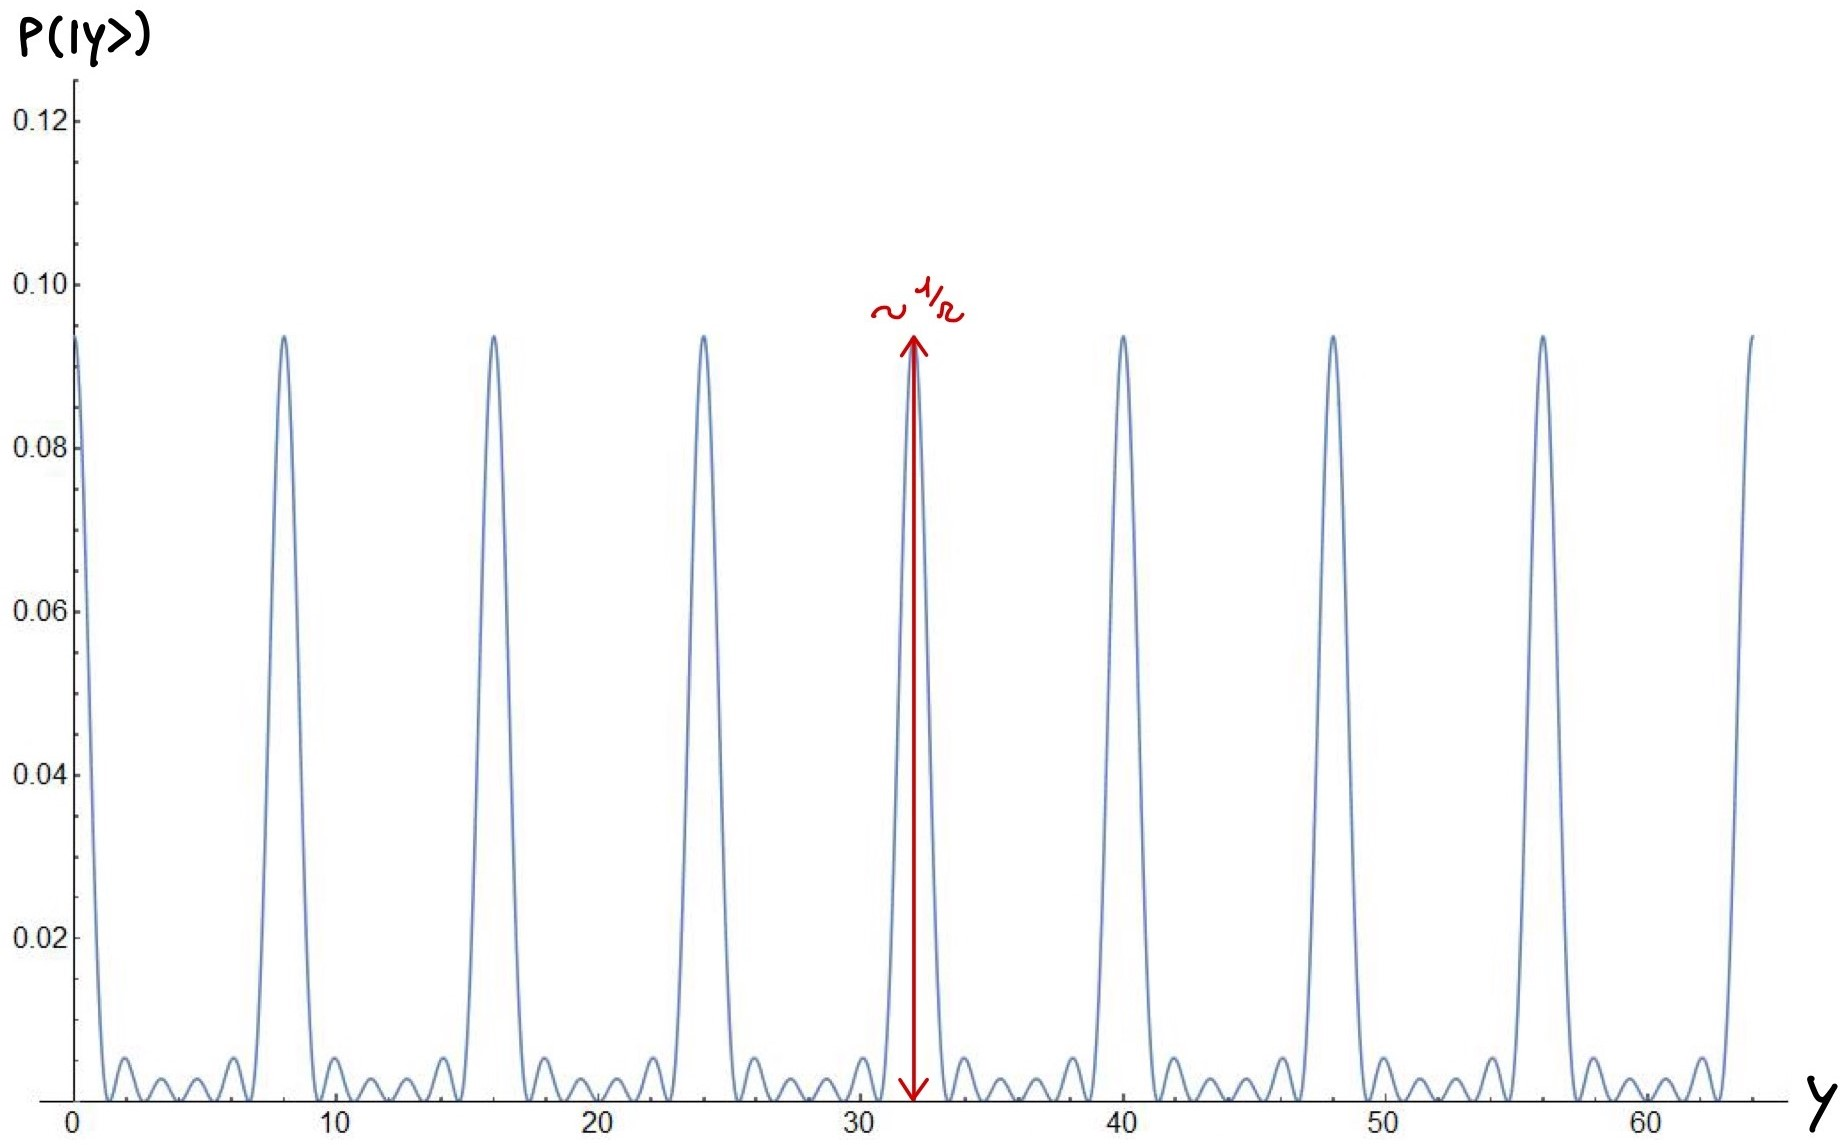
\includegraphics[scale=0.325]{images/probability_y}
    \caption{Esempio di grafico della probabilità di misurare $y$ della formula \eqref{probability_y}, dove $0 \leq y \leq 2^n$. In questo esempio si è usato $n = m = 6$ e $r = 8$. Si noti come il numero di picchi sia $\order{r}$ e la loro altezza, come ordine di grandezza, comparabile a $1/r$.}
    \label{fig:probability_y}
\end{figure}
Notiamo che vi sono differenti picchi di diverse ampiezze: ciò è dovuto al fatto che ci sono valori di $y$ dove abbiamo interferenza costruttiva, mentre in altri si ha interferenza distruttiva. Nel realizzare tale grafico, però, abbiamo assunto che $y \in \mathbb{R}$, ma bisogna ricordare che $y\in \mathbb{Z}$, quindi si tratta di un'approssimazione perché non tutti i punti della curva devono essere disegnati! In realtà, per valori di $n$ molto grandi $2^n$ è enorme quindi la discretizzazione è minima e quasi impercettibile. Nei punti in cui la probabilità è maggiore, in corrispondenza dei picchi più alti, si ha $y = j\frac{2^n}{r}$ dove $j \in \mathbb{N}$. Per tali valori, gli esponenziali dentro la probabilità in \eqref{probability_y} non sono altro che $e^{2\pi i j k}=1$ perché $j, k \in \mathbb{Z}$, quindi la \eqref{probability_y} diventa:
\begin{equation*}
    P(\ket{y}) = \frac{1}{m 2^n} \abs{\sum_{k=0}^{m-1} 1}^2 = \frac{m^2}{m2^n} = \frac{m}{2^n} \, ,
\end{equation*}
il quale è il valore massimo della probabilità. Per capire per quale ragione abbiamo indicato nel Grafico \ref{fig:probability_y} che l'altezza dei picchi è di circa $1/r$, ricordiamo che $2^n \sim N^2$, $r \sim N$ e anche $m \sim N$, per cui:
\begin{equation*}
    P(\ket{y}) = \frac{m}{2^n} \sim \frac N{N^2} \sim \frac 1 N \sim \frac 1 r \, .
\end{equation*}
Notiamo che sebbene abbiamo disegnato una funzione continua, l'approssimazione è comunque molto buona perché la probabilità totale è correttamente normalizzata a 1: infatti l'altezza dei picchi per il loro numero non è altro che $\frac{1}{r} \times m \sim \frac{1}{r} \times r \simeq 1$, quindi gran parte della probabilità è saturata i corrispondenza dei picchi (si può dimostrare che nel limite in cui $n \to \infty$ i picchi tendono a delle delta function). 

\noindent Un risultato fondamentale è che passando attraverso delle manipolazioni algebriche di seno e coseno, si può dimostrare che si ha circa il $40$\% di possibilità ($P(\ket{y}) = \frac{4}{\pi^2}$) di misurare $y$ e ottenere un valore che si trovi in prossimità di uno di questi picchi con un errore di circa $\frac 12$: ricordando che i picchi sono situati in $y = j \frac{2^n}{r}$, possiamo formalmente scrivere che
\begin{equation}
    \abs{y-j\frac{2^n}{r}} < \frac 12 \, , \quad \Rightarrow \quad 
    \abs{\frac y{2^n}-\frac jr} < \frac 1{2^{n+1}} \, ,
    \label{eq:shor2}
\end{equation}
dove abbiamo diviso per $2^n$. Stiamo quindi dicendo che una misura di $y$ soddisfa la disuguaglianza \eqref{eq:shor2} il 40\% delle volte. Possiamo estrarre $r$ dalla \eqref{eq:shor2}? Innanzitutto notiamo che, essendo $0 \leq y \leq 2^n$, abbiamo $0 \leq \frac{y}{2^n} \leq 1$. Se $n \geq 2 n_0$ allora avremo $2^{n}\geq 2^{2n_0}=N^2$, quindi quando la \eqref{eq:shor2} è verificata esiste un singolo numero razionale della forma $\frac j r$ che la  soddisfa e dalla quale è possibile estrarre $r$. 

\noindent La logica è mostrata nel disegno della Figura \ref{fig:inequality_40}: prendendo il segmento $[0,1]$ e suddividendolo in step uguali di lunghezza $\frac{1}{2^n}$, possiamo rappresentare con delle barrette verticali tutti i possibili valori di $y$ tali che $0 \leq \frac{y}{2^n} \leq 1$. La disuguaglianza \eqref{eq:shor2} ci dice che il numero $\frac{j}{r}$ (indicato con una "$\times$" azzurra) è vicino a $\frac{y}{2^n}$ con una distanza minore di $\frac{1}{2^{n+1}}$. 
\begin{figure}[!ht]
    \centering
    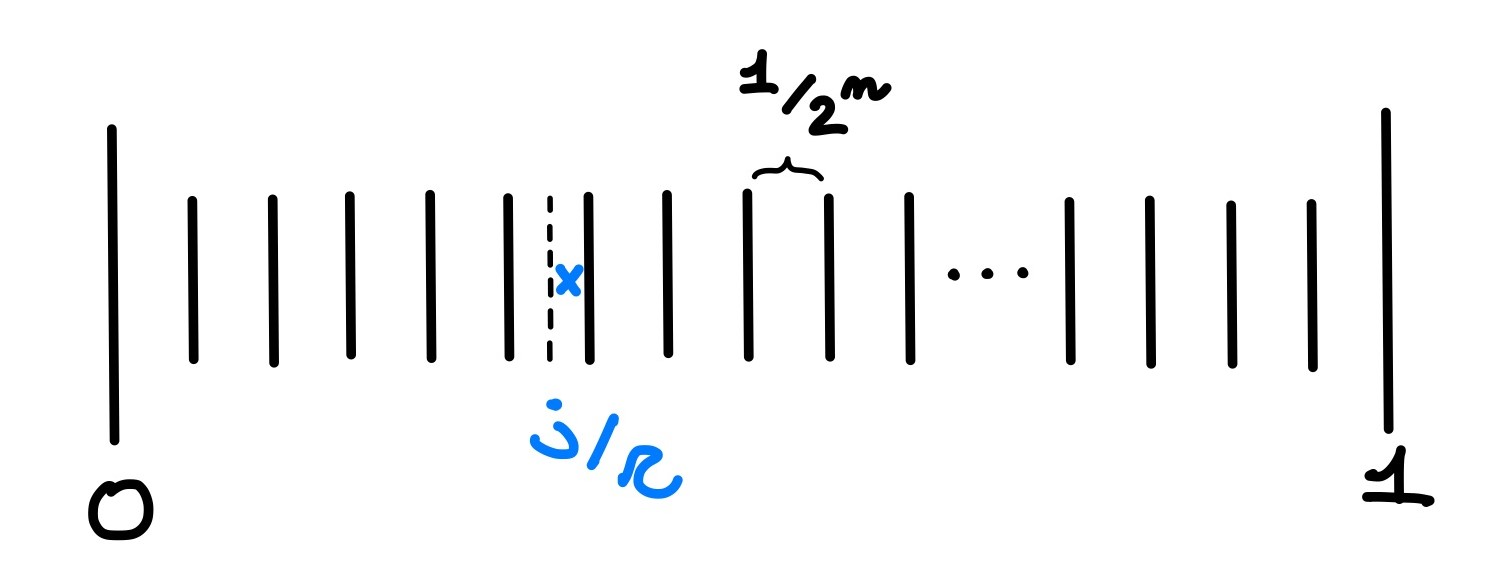
\includegraphics[scale=0.3]{images/inequality_40}
    \caption{Rappresentazione geometrica della disuguaglianza \eqref{eq:shor2}.}
    \label{fig:inequality_40}
\end{figure}

\noindent La domanda che possiamo porci è se esista più di un numero razionale che soddisfi questa particolare proprietà. Supponiamo per assurdo che esistano due numeri razionali $\frac{j_1}{r_1}$ e $\frac{j_2}{r_2}$ che soddisfano la disuguaglianza \eqref{eq:shor2} (e la condizione per cui $r_1, r_2 < N$). Allora la differenza tra questi due numeri è
\begin{equation}\label{difference_rational_numers}
    \frac{j_1}{r_1} - \frac{j_2}{r_2} = \frac{r_2j_1-r_1j_2}{r_1r_1} \, ,
\end{equation}
tuttavia il numeratore è un intero e il denominatore è di ordine $\order{N^2}$: essendo $r_1, r_2 < N$ allora il denominatore è strettamente minore di $N^2$ quindi la \eqref{difference_rational_numers} è $\geq \frac 1{N^2} \geq \frac{1}{2^n}$, che è proprio la larghezza degli step in cui abbiamo suddiviso $[0,1]$. Questo significa che se ci sono due soluzioni della \eqref{eq:shor2} allora la distanza tra le due deve necessariamente essere più grande della misura dello step: in un dato step è possibile trovare una sola soluzione, ossia un solo numero razionale che verifica la \eqref{eq:shor2}.

\noindent Riassumendo: misurando un valore $y$ che soddisfa la \eqref{eq:shor2} otteniamo un unico numero razionale $\frac{j}{r}$. Il punto chiave è quindi trovare  $\frac jr$, tuttavia questo non è così semplice, perché quello che si ottiene dalla misura è un numero scritto in forma decimale, il quale vorremmo poterlo scrivere come rapporto tra razionali. Nonostante ciò facciamo uso del seguente risultato di teoria dei numeri che non dimostreremo. Usando $\frac{1}{2^{n+1}} \leq \frac{1}{2 N^2}\leq \frac{1}{2 r^2}$, riscriviamo la disuguaglianza \eqref{eq:shor2} come
\begin{equation*}
    \abs{x-\frac jr} \leq \frac 1{2r^2} \, , \; \text{ dove } x\in[0,1] \, .
\end{equation*}
Il valore $x$ è dato dalla misura mentre lo scopo è quello di trovare un numero razionale $\frac jr$ che soddisfi questa disuguaglianza. Il risultato dalla teoria dei numeri asserisce che questo valore appare nell'espansione in frazione continua del numero $x$:
\begin{equation*}
    x=\frac{1}{x_0+\frac{1}{x_1+\frac{1}{x_2+\ldots}}} \, .
\end{equation*}

\begin{esempio}[Espansione in frazione continua]
    Supponiamo di considerare il numero $x=0.256789$. Prendendone l'inverso avremo $\frac{1}{x} = \frac{1}{0.256789} = 3.8942478 \ldots$. Da questo risultato è evidente che $x_0 = 3$. Nello step successivo si calcola $x_1$: calcoliamo $\frac{1}{x}-3$ e poi $\left( \frac{1}{x}-3 \right)^{-1}$, la cui parte intera è $x_1$. Iterando all'infinito questo procedimento si ottiene l'espansione in frazione continua di $x$:
    \begin{equation*}
        x=\frac{1}{3+\frac{1}{1+\frac{1}{8+\dots}}} \, .
    \end{equation*}
    Ad ogni step si ottiene quindi un'approssimazione razionale di $x$, infatti il set di numeri razionali che approssimano il suo valore è dato da $\left\{ \frac 13, \frac 14, \frac 9{35}, \frac {19}{74}, \frac{104}{405}, \dots \right\}$. Più si procede, meglio approssimato sarà il valore di $x$. Il teorema ci dice che a un certo punto possiamo trovare il valore di $\frac jr$ all'interno di questo insieme e questo con una probabilità del 100\%. 
\end{esempio}

\noindent Tuttavia di questo procedimento vanno fatte delle opportune precisazioni:
\begin{itemize}
    \item Supponiamo che $j$ e $r$ abbiano dei fattori comuni (e questo ovviamente non lo sapremo mai), allora il valore di $r$ può essere diverso, infatti:
    \begin{equation*}
        \frac jr=\frac{j_0k}{r_0k}=\frac{j_0}{r_0} \, ,
    \end{equation*}
    quindi mediante la procedura sopraelencata, al posto di trovare il periodo cercato, si ottiene $r_0$. Nonostante ciò si è trovato un divisore di $r$, quindi prendendo la forma analitica di $f$ si può provare a calcolare $f(x+r_0)$, $f(x + 2 r_0)$, $f(x + 3 r_0)$, \dots fino a quando effettivamente si trova un valore uguale a  $f(x)$.
    
    \item Talvolta si possono misurare dei valori $y$ che non soddisfano la disuguaglianza \eqref{eq:shor2} (la probabilità di soddisfarla è infatti del 40\%). In tal caso basta semplicemente ricominciare l'algoritmo da capo con una nuova esecuzione del circuito e della QFT fino a quando non si ottiene un valore di $y$ che soddisfi la \eqref{eq:shor2}. Inoltre è possibile dimostrare che la probabilità che la \eqref{eq:shor2} sia soddisfatta cresce fino al 90\% se si sa a priori che $r < \frac N2$.
\end{itemize}
Concludiamo la discussione dicendo che lo stesso tipo di algoritmo può essere utilizzato per calcolare i \textit{logaritmi discreti}, oppure per la simulazione di sistemi quantistici (si possono calcolare gli autovalori di matrici unitarie molto grandi che servono per il calcolo degli autovalori delle relative hamiltoniane e degli evoluti temporali).